% !TEX root = ../main.tex
\graphicspath{{./figures/}}

%%%%%%%%%%%%%%%%%%%%%%%%
\chapter{Implementation}
\label{chap:implementation}
%%%%%%%%%%%%%%%%%%%%%%%%

The design above allows for multiple implementations, which will be introduced in this section. This section will also discuss briefly the robustness of the implementations, meaning how they respond to invalid input graphs. This paper will cover three implementations, which were chosen as they promise efficiency and scalability.

The implementations were coded in Python. Python is versatile, simple, and offers a large collection of helpful libraries like NetworkX, a library for working with graphs \cite{hagbergExploringNetworkStructure2008}. 

The algorithms take as input python dictionaries ("dicts"), which map a key to a value \cite{pythonsoftwarefoundationPythonTutorialSection}. The delegation graph is represented in a "dict of dicts" format, where every key in the outer dict is a node, and the value is another dict, which has the node's delegates as keys, and the weight of the delegation as value. The algorithms use as input "inverse" delegation graphs, where the inner dictionaries represent a node's incoming rather than delegations. \Cref{fig:inverse_dict_example} shows an example of this. Considering that the standing power equations used in the system of linear equations list contain the incoming delegations for each node, this design choice improves efficiency as an algorithm can look up a node in the dictionary and immediately learn about all of its incoming delegations.

\begin{figure}[t]
    \centering
    \begin{subfigure}[t]{0.45\textwidth}
        \centering
        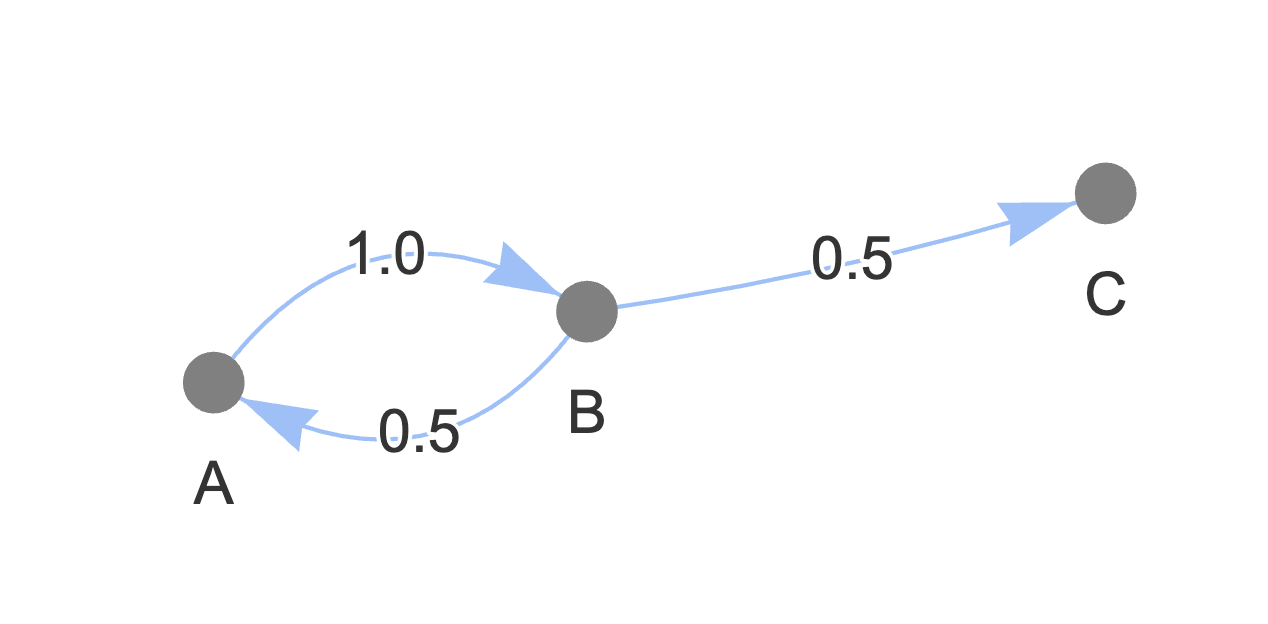
\includegraphics[width=\textwidth]{small_cycle_graph}
        \caption{Delegation graph}
    \end{subfigure}
    \hfill
    \begin{subfigure}[t]{0.45\textwidth}
        \centering
        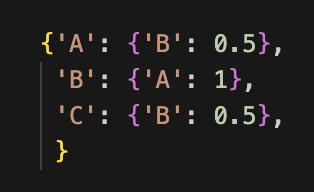
\includegraphics[width=\textwidth]{small_cycle_graph_inverse_dict}
        \caption{Inverse dict representation}
    \end{subfigure}
    \caption{Delegation graph and its inverse dict representation}
    \label{fig:inverse_dict_example}
\end{figure}

\section{Linear Systems Solver}

The first approach uses a dedicated linear system solver. We use SciPy's \texttt{scipy.sparse.linalg.spsolve} solver, which is optimized for sparse matrices \cite{virtanenSciPy10Fundamental2020}. A sparse solver is better equipped to resolve delegations if we assume that realistically each delegator only delegates to a few delegates. Since each entry in matrix $W$ can be mapped to one unique edge $(u, v, p) \in E$, the matrix likely has relatively few non zero entries compared to its size.
 
 The implementation makes use of SciPy's Compressed Sparse Column (CSC) arrays, which builds matrixes using $(x,y)$ coordinates and their corresponding data, which unless explicitly set is 0. \cite{virtanenSciPy10Fundamental2020}

The solver solves the system of linear equations directly, using the SuperLU solver, meaning it will always solve the system of linear equations perfectly accurately, unlike the other implementations discussed below. \cite{liSuperLUUsersGuide1999} The solver's results are then cleaned, setting each node with outgoing edges', so each delegator's, power to zero, and returned.

The implementation will be referred to as \ac{LS} throughout the paper.

\section{Linear Programming Solver}

Secondly, we use the Python library PuLP, which provides an interface to linear programming solvers \cite{osullivanPuLPLinearProgramming2011}. To resolve the delegation graphs, we use the "Coin-or branch and cut" (CBC) solver, since it is free and open-source \cite{johnforrestCoinorCbcRelease2024}. Given the academic context and the moderate size of our delegation graphs, CBC provides a balance between performance and accessibility. Moreover, since our model essentially solves a system of linear equations with a unique correct solution, the choice of solver has little influence on the outcome itself — even if CBC is not the most optimized solver for this class of problems. While commercial solvers may offer faster runtimes, CBC is sufficient for our use case and ensures reproducibility without licensing constraints.

The algorithm first sets up the linear program, setting up an equation $p'_v = \sum_{(u, v, w) \in E} 1 + wp'_u$ for each node $v \in V$. This is then solved by the CBC solver, with the primal tolerance set to $5*10^{-3}$ to level the playing field compared to the iterative algorithm, which will be introduced in the next section. A tolerance of $5 * 10^{-3}$ assures that $\lvert p'_v -\sum_{(u, v, w) \in E} 1 + wp'_u \rvert \le 5*10^{-3}$, so the solutions will be correct when rounded to the second decimal place \cite{forrestCBCUserGuide2005}. Finally, the algorithm cleans the $p_v'$ values, setting any delegators power to 0. 

The implementation will be referred to as \ac{LP} throughout the paper.

\TODO{Add links to the implementations on GitHub}

\section{Iterative Solver}

The iterative solver aims to leverage the format of the input, and eliminate any necessary overhead. It is based on the Jacobi method of solving systems of linear equations, which solves the system by iteratively refining the solution \cite{burden2011numerical}, however we will prioritize an intuitive explanation of the procedure.

\subsection{Approach}

A delegation can be thought about as liquid throwing through a graph. Each delegator is a "source", and power flows from its source between nodes until it eventually ends in a sink. If a delegator $A$ delegates half their vote to $B$ and the other half to other nodes, half of $A$'s power should flow to $B$. An algorithm should thus add 0.5 to $B$s power, and remove it from $A$. If $B$ is a sink, the algorithm is done resolving this delegation. However, $B$ may not be a sink, in which case, the power continues to flow further, to $B$'s delegates. An algorithm would need to iterate over the graph multiple times, until an equilibrium has been reached, where all power in the graph has flown into a sink. \Cref{alg:iterative_simple} shows such an algorithm drafted in pseudocode. Each iteration, a snapshot of the power's of each node is taken, and the reassignments of power are based on this snapshot\footnotemark.  

\footnotetext{If the algorithm forwent the use of such a snapshot, it would lead to inconsistencies in the edge case of a self-delegation of weight less than 1, since the self-delegator's power would change in the middle of reassigning the power. This is also how the Jacobi method approaches this challenge. Each iteration, a solution vector containing intermediate results is created, and passed as input into the next iteration.}

Another valid approach would be a queue-approach, where the algorithm pops node off a queue and delegates their power, and each delegate of this node gets re-added to the queue. A sweeping method treating the entire graph at once was chosen due to its increased simplicity and runtime analysis.

\begin{algorithm} [t]
 \caption{Iterative algorithm}\label{alg:iterative_simple}
\begin{algorithmic}[1]
\State // Initialize each node’s power to 1.0  
\ForAll{\(v \in \texttt{nodes}\)}
    \State \(\texttt{powers}[v] \gets 1.0\)
\EndFor
\Repeat
    \State \(\texttt{prev\_powers} \gets \texttt{powers}.\texttt{copy}()\)  \Comment{snapshot of previous iteration}
    \ForAll{\(v \in \texttt{nodes}\)}
        \State // For each incoming delegation \((u \to v)\), move \(w_{uv}\times\) previous power of u
        \ForAll{\((u, w) \in \texttt{delegations}[v]\)}
            \State \(\delta \gets w \times \texttt{prev\_powers}[u]\) \label{alg:iterative_simple_delta_assignment}
            \State \(\texttt{powers}[u] \;-\!=\; \delta\) \label{alg:iterative_simple_remove_delta}
            \State \(\texttt{powers}[v] \;+\!=\; \delta\) \label{alg:iterative_simple_add_delta}
        \EndFor
    \EndFor
\Until{\(\texttt{prev\_powers} = \texttt{powers}\)} \label{alg:iterative_simple_termination_cond}\Comment{a steady state has been reached}
\end{algorithmic}
\end{algorithm}

The following notation will be used throughout the next sections.

$G = (V, E)$ is a well-formed delegation graph, with $V = D \dot\bigcup S$, where D is the set of delegators and S is the set of sinks.

Let $p_v^{(i)}, i \in \mathbb{N}_0$ be \texttt{powers}[v] after the $i$-th iteration of the repeat-until loop, with $p_v^{(0)}$ being the initial power of a node before the first iteration has started. Using this notation, our termination condition for the repeat-until loop of \cref{alg:iterative_simple} is: $\forall v \in V: p_v^{(i-1)} = p_v^{(i)}$

Let $P_D^{(i)} = \sum_{d \in D} p_d^{(i)}$ and $P_S^{(i)} = \sum_{s \in S} p_s^{(i)}$ be the sums of the power values all delegators and all sinks after each iteration.

Let $\delta_{(u, v, w)}^{(i)} = w * p_v^{(i)}$ be the delta assigned in line 10 of \cref{alg:iterative_simple} during the $i$th iteration.

\subsection{Conservation of Power}

We show, that this algorithm conserves power throughout iterations.

\begin{theorem}
\label{theo:iterative_cons_of_power}
Given a well-formed delegation graph, in \cref{alg:iterative_simple}, $P_t^{(i)} = P_D^{(i)} + P_S^{(i)}$ is equal to $|V|$ for any $i \in \mathbb{N}_0$.
\end{theorem}
\begin{proof}

We prove the theorem inductively. When $i = 0$ (before the first iteration), each node is assigned a power of 1. So 

\[
\forall v \in V: p_v^{(0)} = 1 \implies P_t^{(0)} = |V|
\]

Assume that for a $k \in \mathbb{N}_0: P_t^{(k)} = |V|$. During iteration $k+1$, the algorithm will iterate over all delegations, and for each $(u, v, w) \in E$, it will remove some $\delta_{(u, v, w)}^{(k+1)}$ from node \texttt{u}, but add this same amount to node \texttt{v}. Since the delegation graph is well formed, the outgoing weights of any delegator add up to 1, so for all delegators $u \in D$, the total amount of power they delegate away during iteration $k+1$ adds up to the power they held in iteration $k$. Formally, for any node $u \in V$:

\begin{align*}
\sum_{(u, v, w) \in E} \delta_{(u, v, w)}^{(k+1)} &=  \sum_{(u, v, w) \in E} wp_u^{(k)} \\
&= p_u^{(k)}  \cdot \sum_{(u, v, w) \in E} w \\
&= p_u^{(k)} \cdot 1 \\
&= p_u^{(k)}
\end{align*}

Thus, throughout the iteration of the outer loop, any delegator $u$ only ever moves power it already has, and for each "moving around" of power, conservation is guaranteed since any power subtracted from a delegator is re-added to the delegate. Thus $P_t^{(k+1)} = |V|$. 

By the principles of induction, the assumption holds for any $i \in \mathbb{N}_0$

\end{proof}

\subsubsection{Similarity to the Previous Approach}

Observing the algorithm reveals that the same equations used in the previous approach to resolve delegations can be re-found here. The algorithm starts with a vector of ones, indicating an initial power of each node of one. Furthermore, each iteration, each node $u \in V$ gains power amounting to $\sum_{(u, v, w) \in E} \delta^{(i)}_{(u, v, w)}$. This can be rearranged as follows:

\begin{align*}
p_v^{(i)} &+= \sum_{(u, v, w) \in E} \delta^{(i)}_{(u, v, w)} \\
&+= \sum_{(u, v, w) \in E} wp_v^{(i-1)}
\end{align*}

Since power is conserved, any power node $u$ held from the previous iteration $i - 1$ is delegated away during iteration $i$, thus we can say, that

\[
p_v^{(i)} = \sum_{(u, v, w) \in E} wp_v^{(i-1)} \forall v \in V
\]


This is the same al the standing power assigned to all nodes in the previous approach. ($p'_v = 1 + \sum_{(u, v, w) \in E} wp'_u$). Thus, this algorithm solves the same problem as the system of linear equations introduced in the previous section. 

This section will show, that the algorithm does not necessarily terminate despite being input a well formed delegation graph. We then propose an amended algorithm.

We first prove that the algorithm terminates at iteration $i+1$ exactly when $P_D^{(i)} = 0$.

\begin{lemma}\label{lem:simple_alg_terminates}
 $p_v^{(i)} = p_v^{(i+1)} \forall v \in V \Leftrightarrow$ $P_D^{(i)} = 0$.
\end{lemma}
\begin{proof}

\begin{align*}
	P_D^{(i)} = 0 
	&\Leftrightarrow p_d^{(i)} = 0, \forall d \in D \\
	&\Leftrightarrow \not\exists (d, v, w) \in E: \delta_{(d, v, w)}^{(i+1)} > 0  &&\text{($\delta$ of a node with power 0 is 0)}\\
	&\Leftrightarrow p_v^{(i)} = p_v^{(i+1)} \forall v \in V \qed  &&\text{($p_v$ doesn't change if zero is added to it)}
\end{align*}
\end{proof}

This insights lets us prove, that the algorithm may never terminate.

\begin{theorem}\label{alg:iterative_alg_doesnt_terminate}
Given a well-formed delegation graph, \cref{alg:iterative_simple} may not terminate.
\end{theorem}
\begin{proof} 

Assume the algorithm terminates on a well-formed delegation graph..

Take the following well formed delegation graph $G = (S \dot\bigcup D, E)$ with $S =\{C\}$ and $D = \{A, B\}$, visualized in \cref{fig:small_cycle_graph}. Since the algorithm terminates, there must be an $i \in \mathbb{N}$ such that $P_D^{(i)} = 0$ (\cref{lem:simple_alg_terminates}). 

\begin{figure}[t]
    \centering
    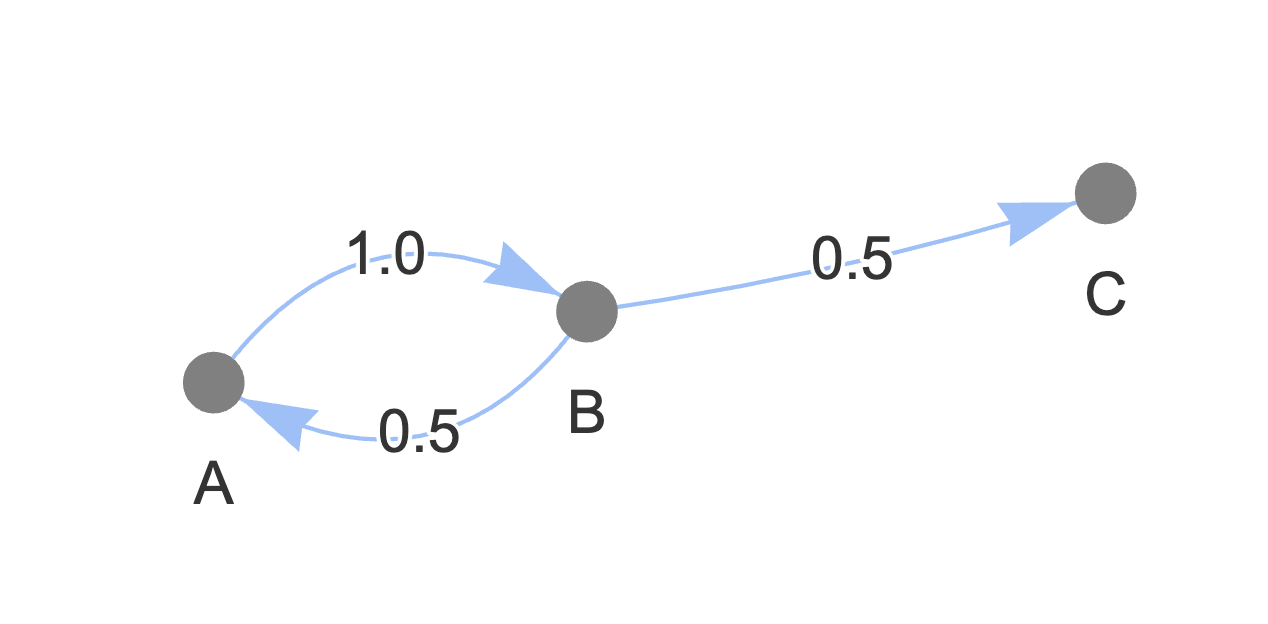
\includegraphics[width=0.4\textwidth]{small_cycle_graph}
    \caption{Delegation graph with a cycle}
    \label{fig:small_cycle_graph}
\end{figure}

In each iteration $i$, half of $B$’s power is passed to $A$, which immediately returns it in the next iteration. This creates an infinite back-and-forth delegation loop between $A$ and $B$, where power keeps circulating and leaking only partially to the sink $C$. 

The power values of the three nodes as the algorithm iterates are shown in \cref{tab:simple_iterative_example}. The power values for $A$ and $B$ decrease, but never reach zero, which implies that:

\[
\forall i: P_D^{(i)} > 0
\]

\end{proof}

\begin{table}[t]
  \centering
  \caption{$p_v{(i)}$ values of nodes in the graph in \cref{fig:small_cycle_graph}}
  \label{tab:simple_iterative_example}
  \begin{tabular}{| l | l | l | l |}
    \hline
    i & $p_A$ & $p_B$ & $p_C $ \\ \hline
    0 & 1 & 1 &	1 \\ \hline
    1 & 0.5 & 1 & 1.5 \\ \hline
    2 & 0.5 & 0.5 & 2 \\ \hline
    3 & 0.25 & 0.5 & 2.25 \\ \hline
    4 & 0.25 & 0.25 & 2.50 \\ \hline
    5 & 0.125 & 0.25 & 2.625 \\ \hline
    \multicolumn{4}{| l |}{...} \\ \hline
  \end{tabular}
\end{table}

Practically, the algorithm needs a cutoff condition, which terminates the repeat-until loop once the power values calculated are close enough to the real, final values. Since these are unknown before the algorithm terminates, we can count how much power is being shifted throughout the graph each iteration, and terminate once this value is sufficiently small. An extension to \cref{alg:iterative_simple} could look like \cref{alg:iterative_with_cutoff}. We now show that is also conserves power, and that it terminates.

\begin{algorithm} [t]
 \caption{Iterative Algorithm with a cuttoff value. Changes from \cref{alg:iterative_simple} are highlighted.}\label{alg:iterative_with_cutoff}
\begin{algorithmic}
\State // Initialize each node’s power to 1.0  
\ForAll{\(v \in \texttt{nodes}\)}
    \State \(\texttt{powers}[v] \gets 1.0\)
\EndFor
\Repeat
    \State \(\texttt{prev\_powers} \gets \texttt{powers}.\texttt{copy}()\) 
    \State \colorbox{yellow}{\(\texttt{total\_change} \gets \texttt{0}\)} 
    \ForAll{\(v \in \texttt{nodes}\)}
        \State // For each incoming delegation \((u \to v)\), move \(w_{uv}\times\) previous power of u
        \ForAll{\((u, w) \in \texttt{delegations}[v]\)}
            \State \(\delta \gets w \times \texttt{prev\_powers}[u]\)
            \State \(\texttt{powers}[v] \;+\!=\; \delta\)
            \State \(\texttt{powers}[u] \;-\!=\; \delta\)
            \State \colorbox{yellow}{\(\texttt{total\_change} \;+\!=\; \delta \)}
        \EndFor
    \EndFor
\Until{\colorbox{yellow}{\(\texttt{total\_change} < \texttt{cutoff}\)}}
\end{algorithmic}
\end{algorithm}

\subsubsection{Conservation of Power}

\Cref{theo:iterative_cons_of_power} states that \cref{alg:iterative_simple} conserves power across iterations. The same proof applies to \cref{alg:iterative_with_cutoff}, since only the if-condition of the outer loop has changed, but the algorithm works the same way. So while the algorithm will iterate less, power remains conserved across iterations.

\subsubsection{Termination}

\begin{lemma}\label{lem:iterative_alg_power_concentrates}
Given a well-formed delegation graph, \cref{alg:iterative_with_cutoff} terminates if $\texttt{cutoff} > 0$.
\end{lemma}
\begin{proof}

For this proof, we use the fact that this method of resolving delegation essentially implements the Jacobi method for solving linear equations. In the Jacobi method, the system of linear equations is iteratively refined as follows. Note, that we use the matrix representation of the system of linear equations from \cref{subsec:unique_sol}.

\[
p_{(i + 1)} = Wp_{(i)} + 1
\]

$p_{(i)}$ is the vector of power values after iteration $i$. Unfolding this recursive equation, with $p_0 = \mathbb{1} $, the vector of ones, yields:

\begin{align*}
p^{(1)} &= W p^{(0)} + \mathbb{1} \\
p^{(2)} &= W p^{(1)} + \mathbb{1} = W(W p^{(0)} + \mathbb{1}) + \mathbb{1} = W^2 p^{(0)} + W \mathbb{1} + \mathbb{1} \\
p^{(3)} &= W p^{(2)} + \mathbb{1} = W^3 p^{(0)} + W^2 \mathbb{1} + W \mathbb{1} + \mathbb{1} \\
\vdots \\
p^{(n)} &= W^n p^{(0)} + \sum_{k=0}^{n-1} W^k \mathbb{1} \\
\end{align*}


Since the system of linear equations has a unique solution, as proven in \cref{subsec:unique_sol}, we know that matrix $\rho(W) < 1$. This implies, that:

\[
\lim_{k \to \infty} W^k = 0 \quad \text{and} \quad \sum_{k=0}^{\infty} W^k = (I - W)^{-1}
\]

Thus, $p^{(n)}$ converges. This means, that the changes in power per iteration must shrink strictly monotonically, meaning the \texttt{total\_change} shrinks strictly. Thus, it will eventually fall under the \texttt{cutoff} and the algorithm terminates. 

\end{proof}

\section{Robustness}

This section describes the different implementations behavior when a delegation graph is not well formed. Specifically, their behaviors when outgoing delegation weights are invalid, so not adding up to 1, and if the delegation graph contains a closed delegation cycle. 

\subsection{Invalid delegations}

On their own, neither of the three implementations will definitively cause an error when delegations are invalid. The iterative implementation is "dumb", in the sense that it moves around power as it finds them in the delegations. If a delegator delegates more than they are meant to, the algorithm behavior becomes undefined, since the delegators power may become negative, at which point the delta in power calculated from its power also becomes negative, which messes with the \texttt{total\_change} value in unpredictable ways. 

If a delegate delegates less than their vote, this causes less of an issue. As long as the delta calculated at $\delta \gets w \times \texttt{prev\_powers}[u]$ does not become negative, the algorithm's will still find the power correctly. A well-formed delegation graph is allowed to contain self-delegations as long as their weight is lower than 1, such as the delegation in \cref{subfig:permissible-self-delegation}. In this situation, power still leaves the node, but less slowly. When the iterative algorithm goes over the graph, not delegating enough weight has the same effect as such a self-delegation, since in the former situation  power gets subtracted and then re-added to the node, while in the latter it just remains untouched. Thus, the two graphs in \cref{fig:small-delegation-graphs} yield the same result, $B$ having a power of 2.

\begin{figure}[t]
    \centering
    \begin{subfigure}[t]{0.45\textwidth}
	\centering
	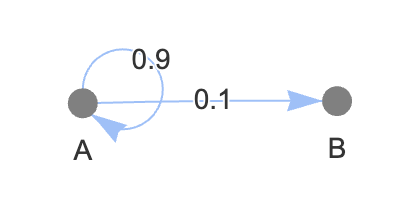
\includegraphics[width=0.9\textwidth]{allowed_self_loop}
	\caption{Permissible delegation graph}
	\label{subfig:permissible-self-delegation}
    \end{subfigure}
    \hfill
    \begin{subfigure}[t]{0.45\textwidth}
        \centering
        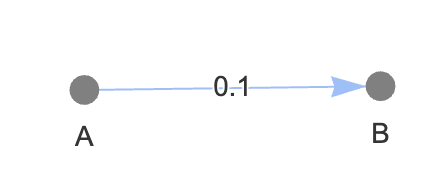
\includegraphics[width=\textwidth]{invalid_delegation_graph}
        \caption{Invalid delegation graph}
         \label{subfig:invalid-delegation-graph} 
    \end{subfigure}
    \caption{Two similar delegation graphs}
    \label{fig:small-delegation-graphs}
\end{figure}

For the two implementations directly based on solving systems of linear equations, this is different. Node \texttt{B}'s power would end up as 1.1, since the system of linear equations looks as follows:

\begin{align*}
& p_A = 1 \\
& p_B = 1 + 0.1p_A
\end{align*}

As long as the delegations form a matrix that is singular, there will be a unique solution, so even with invalid delegations, the algorithm will find power values, however they most likely differ whom the power values that would be expected, and probably not conserve total power properly. 

\subsection{Closed Delegation Cycles}

If the delegations form a closed delegation cycle, the iterative algorithm will not terminate, since the algorithm will iterate any power that is in or enters the cycle around the cycle indefinitely. 

For the other two algorithms however, such a cycle can be caught. The equations for the standing power of the nodes within the cycle are linearly dependent on each other, thus the matrix resulting from them is not singular, and hence don't have a single solution. Solvers of systems of linear equations catch this and throw an error. Similarly, the LP solver will find that the linear program is infeasible.

What is worth mentioning however, is that since we allow fractional delegation, it suffices if just one node in a closed delegation cycle decides to delegate to a node outside of a delegation cycle (or turns into a sink), for the delegations to become resolvable again. The cycles that will be explored in \cref{subsec:cycles_draining} are example of such a situation. 
